\documentclass[a4paper,landspace]{article}
\usepackage[paperwidth=14.13in, paperheight=9.86in]{geometry}
%% \usepackage{geometry}

\usepackage[usenames,dvipsnames]{xcolor}
\usepackage[utf8]{inputenc}
\usepackage{fontspec}
\usepackage{tikz}
\usetikzlibrary{positioning}
\usepackage{rotating}
\usepackage[absolute,overlay]{textpos}
%% Useful to print in an A4/A3 sheet and see the actual size of paper
%% \usepackage[frame,a3,landscape,pdftex,center]{crop}

% donot indent first line of paragraph.
\setlength{\parindent}{0pt}
\setlength{\parskip}{5pt plus 2pt minus 1pt}

\sloppy

%% Completely remove hyphenation
\usepackage[none]{hyphenat}
\usepackage[most]{tcolorbox}
\usepackage{setspace}

\begin{document}
\newfontfamily{\cabinbold}
              [ Path = ../fonts/,
                UprightFont = Cabin-Bold.ttf,
              ]{ Cabin }
\newfontfamily{\dejavusans}
              [ Path = ../fonts/,
                UprightFont = DejaVuSans.ttf,
                BoldFont = DejaVuSans-Bold.ttf,
              ]{ DejaVu Sans }
\newgeometry{top=0cm, bottom=0cm}
\pagestyle{empty}
\pagecolor{Blue}

\begin{textblock*}{0in}(6.97in,0.5in) % {block width} (coords)
  \begin{turn}{-90}
    {\fontsize{16}{16} {\cabinbold {\color{Yellow} Essentials of Go Programming}}}
  \end{turn}
\end{textblock*}

\begin{textblock*}{0in}(6.99in,5.0in) % {block width} (coords)
  \begin{turn}{-90}
    {\fontsize{14}{14} {\cabinbold {\color{White} First Edition}}}
  \end{turn}
\end{textblock*}

\begin{textblock*}{0in}(6.97in,7.5in) % {block width} (coords)
  \begin{turn}{-90}
    {\fontsize{16}{16} {\cabinbold {\color{White} Baiju Muthukadan}}}
  \end{turn}
\end{textblock*}

\begin{textblock*}{5in}(8in,1.7in) % {block width} (coords)
    {\fontsize{50}{50} {\cabinbold {\color{Yellow} Essentials of}}}
\end{textblock*}

\begin{textblock*}{5in}(8in,2.5in) % {block width} (coords)
    {\fontsize{58}{58} {\cabinbold {\color{Yellow} Go Programming}}}
\end{textblock*}

\begin{textblock*}{5in}(10.8in,3.59in) % {block width} (coords)
    {\fontsize{36}{36} {\cabinbold {\color{White} First Edition}}}
\end{textblock*}

\begin{textblock*}{5in}(8.25in,4.4in) % {block width} (coords)

%% Credit: https://commons.wikimedia.org/wiki/File:The_ladder_of_life_is_full_of_splinters.jpg
\tcbox{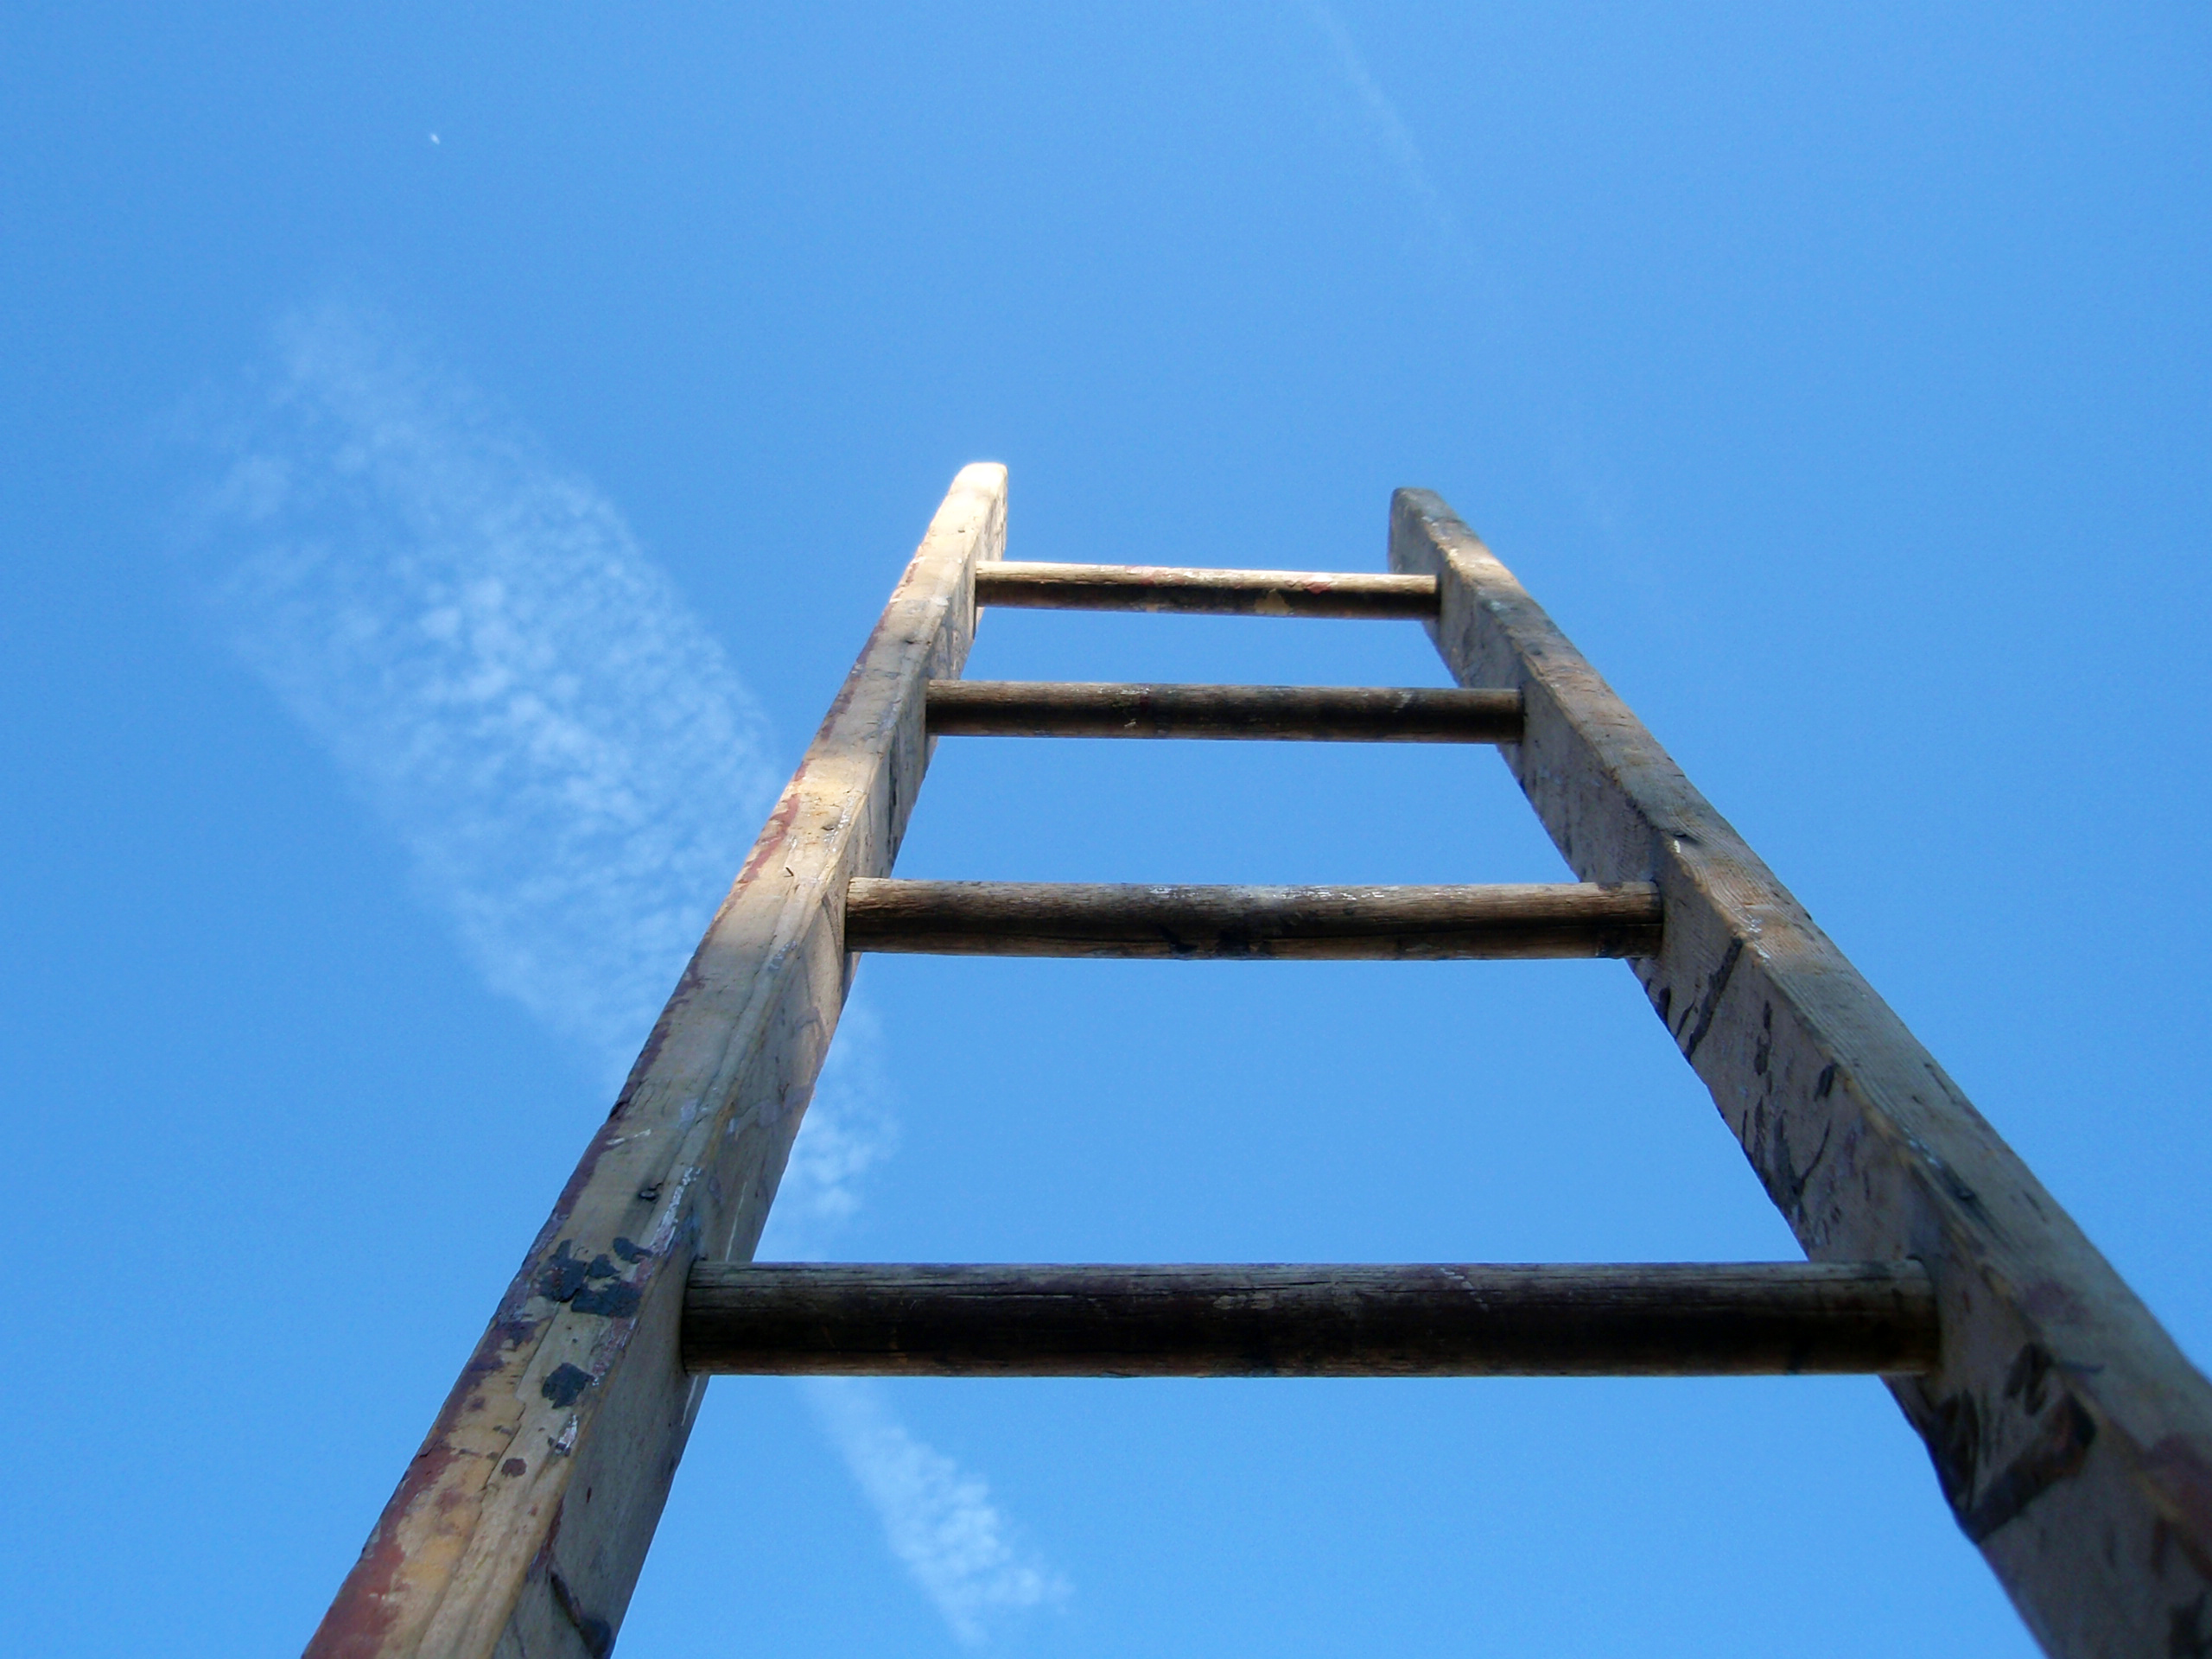
\includegraphics[width=4.7in,keepaspectratio]{images/ladder.jpg}}

\end{textblock*}

\begin{textblock*}{5in}(8.59in,8.6in) % {block width} (coords)
    {\fontsize{42}{42} {\cabinbold {\color{White} Baiju Muthukadan}}}
\end{textblock*}

\begin{textblock*}{5.6in}(0.5in,0.4in) % {block width} (coords)
  {\fontsize{12}{12}

    {\dejavusans {\setstretch{1.2}\color{White} Computer programming
          skill helps you to solve many real-world problems.
          Programming is a process starting from the formulation of a
          computing problem to producing computer programs (software).
          Computer programming is part of a more extensive software
          development process.

Programming involves analysis, design, and implementation of the
software.  Coding is the activity of implementing software.  Sometimes
coding involves more than one programming language and use of other
technologies.  Learning a programming language is a crucial part of
the skill required for computer programming or software development in
general.

Using a programming language, we are preparing instructions for a
computing machine.  The computing machine includes a desktop computer,
laptop, and mobile phone.

There are many programming languages in use today with different
feature sets.  You should learn to pick the right programming language
for the problem at hand.  Some languages are more suitable for
specific problems.  This book provides an introduction to the Go
programming language.  Studying the Go programming should help you to
make the right decision about programming language choice for your
projects.  If you have already decided to use Go, this book should
give an excellent introduction to Go programming.

Go, also commonly referred to as Golang, is a general-purpose
programming language.  Go was initially developed at Google in 2007 by
Robert Griesemer, Rob Pike, and Ken Thompson.  Go was publicly
released as an open source software in November 2009 by Google.
 }}}
\end{textblock*}

\begin{textblock*}{5in}(1.2in,5.45in) % {block width} (coords)

\begin{tikzpicture}
\draw [Yellow, line width=0.1in, dashed] (0,0) -- (10.3,0);
\end{tikzpicture}
\end{textblock*}

\begin{textblock*}{5.6in}(0.5in,5.8in) % {block width} (coords)
  {\fontsize{12}{12}

    {\dejavusans {\setstretch{1.2}\color{White}Baiju Muthukadan is a software
        engineer from Kerala, India. He began his software development career in
        2002. Over the years, Baiju has contributed to many free and open source
        software projects. In 2007, he authored his first book on Python. Since
        2013, he has been working on various Go projects. His Twitter handle is
        @baijum\\ }}

    {\bf {\dejavusans {\color{White} 
          https://github.com/baijum/essential-go}}} }

\end{textblock*}

\end{document}
